\subsubsection{CI/CD (Github Action)}

CI/CD là
phương pháp tự động hóa
quy trình tích hợp
và triển khai phần mềm.
Phương pháp này giúp
đẩy nhanh tốc độ, giảm thiểu lỗi thủ công
và duy trì độ ổn định cho hệ thống.
GitHub Actions là công cụ CI/CD mạnh mẽ được tích hợp sẵn trên GitHub.

\begin{figure}[H]
\centering
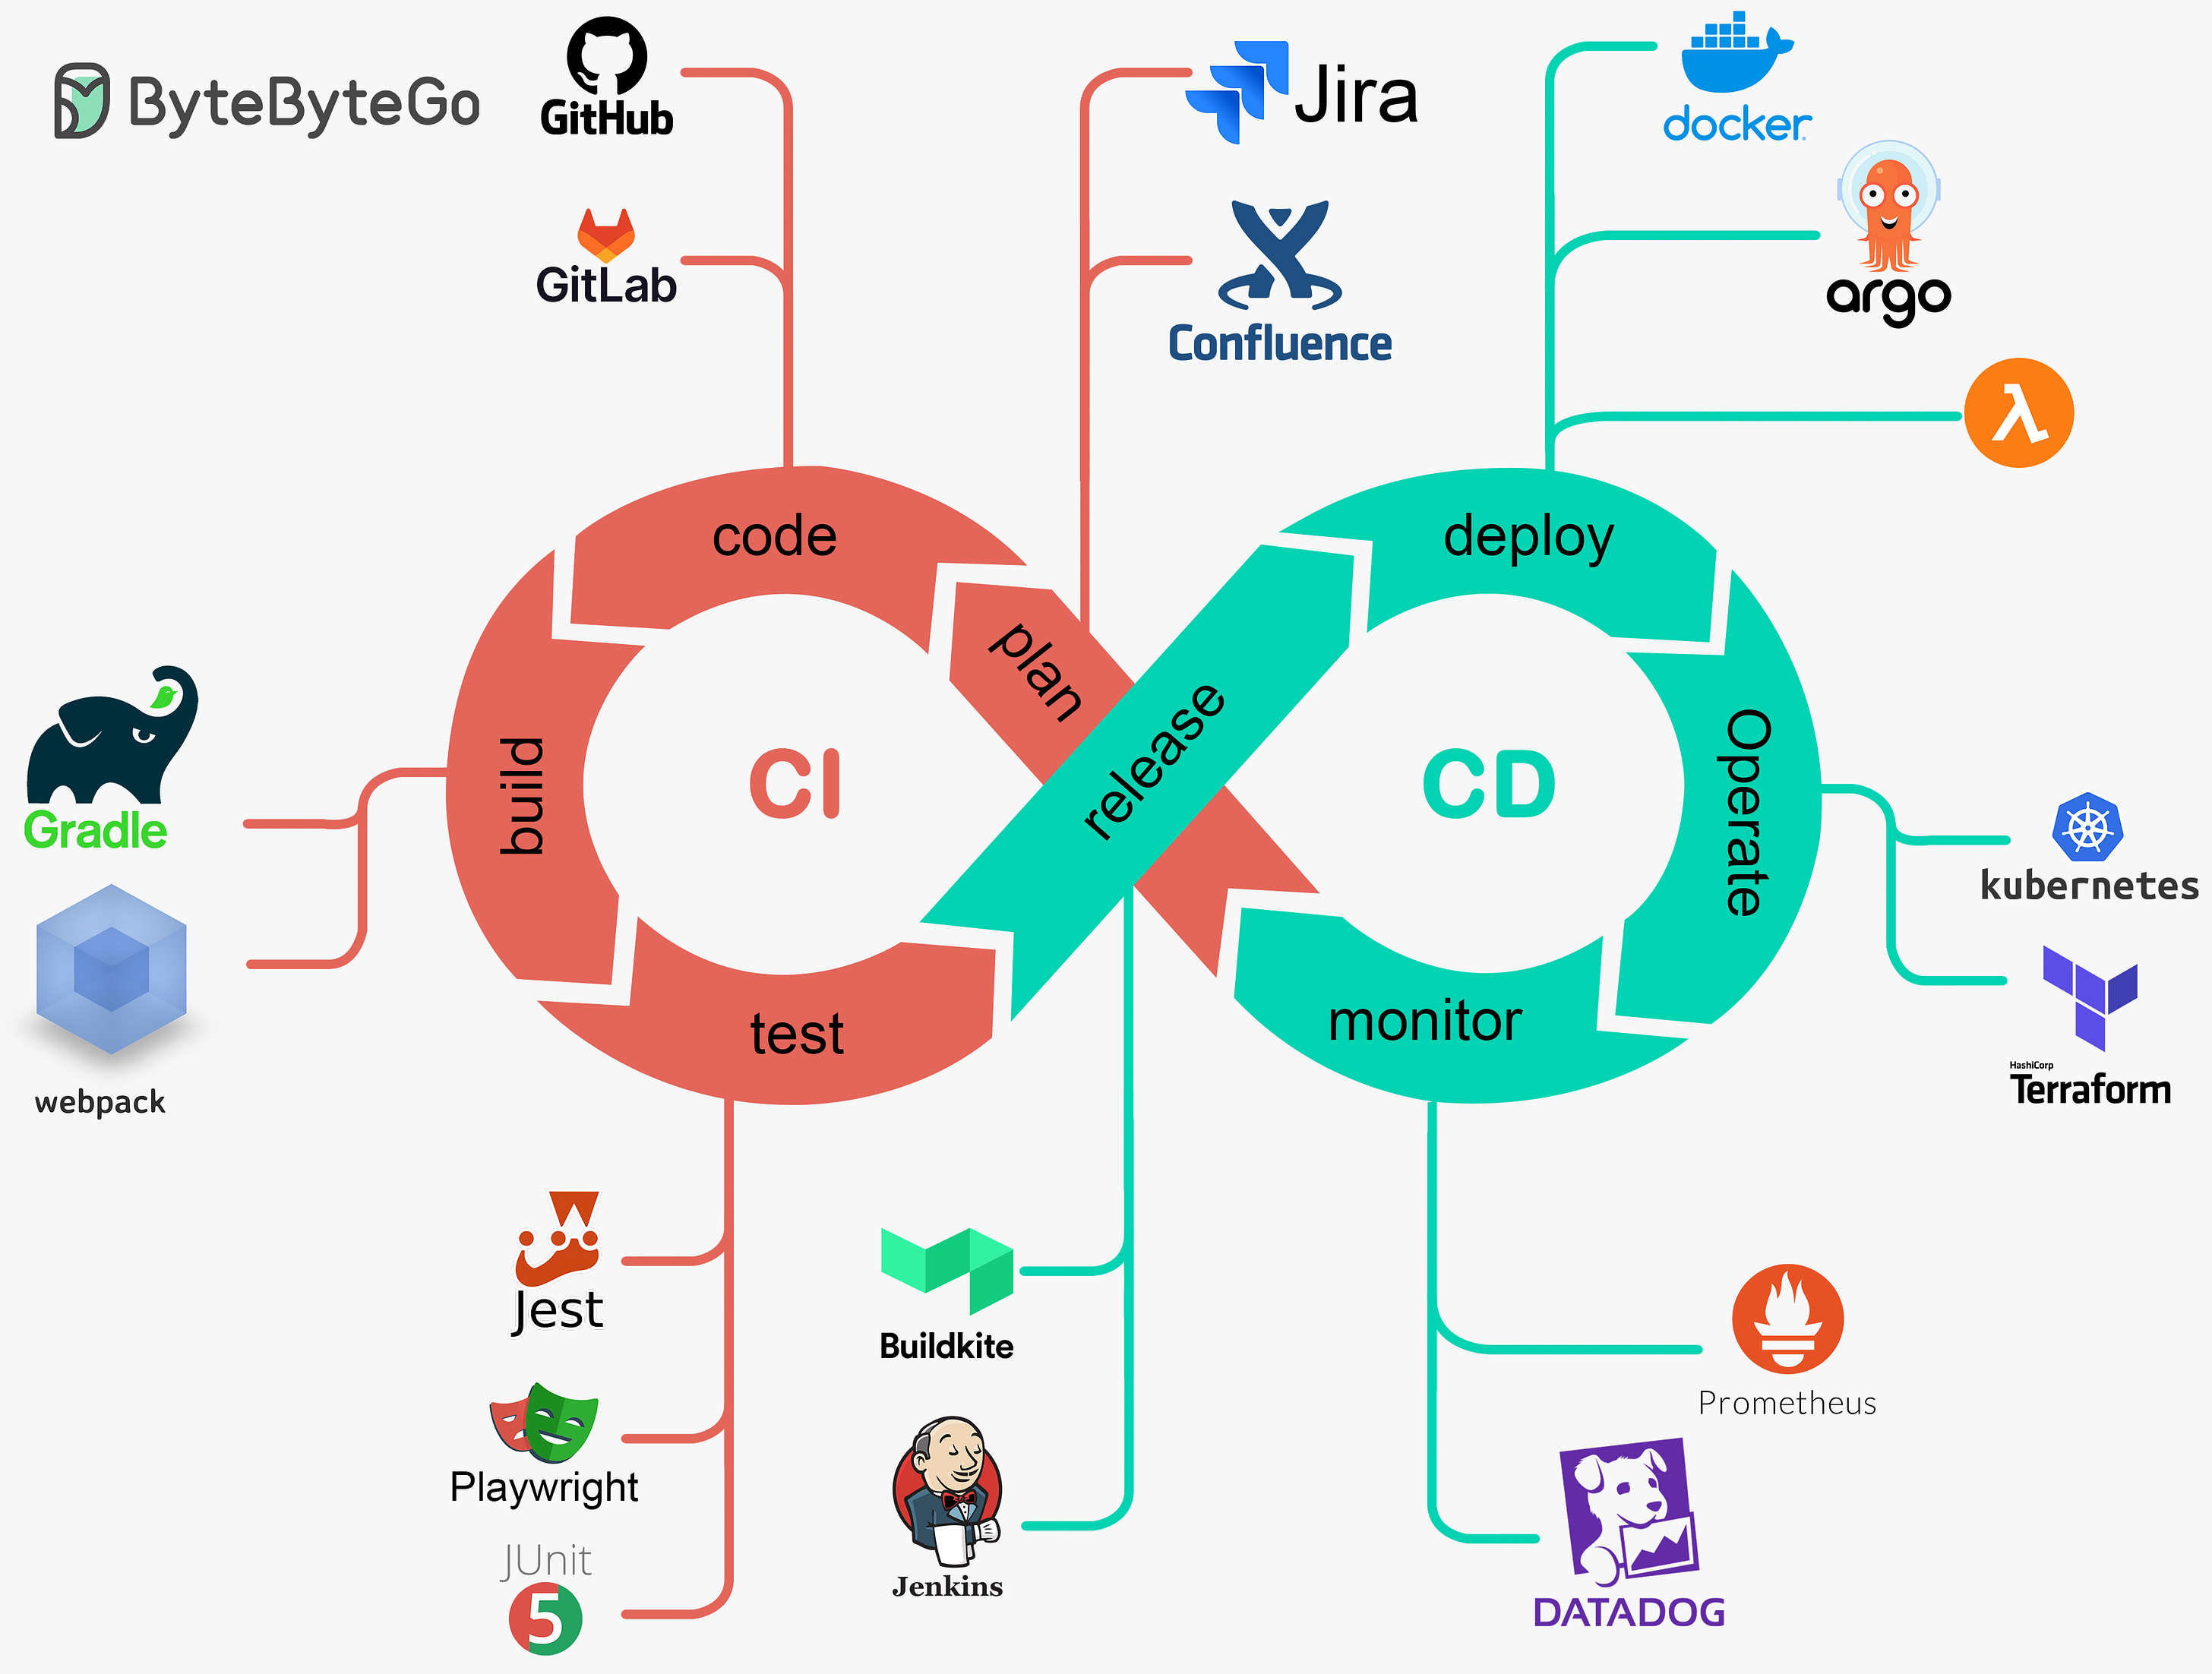
\includegraphics[scale = 0.1]{pictures/cicd-overview.jpg}
\caption{Cấu hình chia nhỏ bí mật theo từng nhu cầu sử dụng trong doppler}
\end{figure}

Sơ đồ CI/CD bằng Github Action

\begin{figure}[H]
\centering
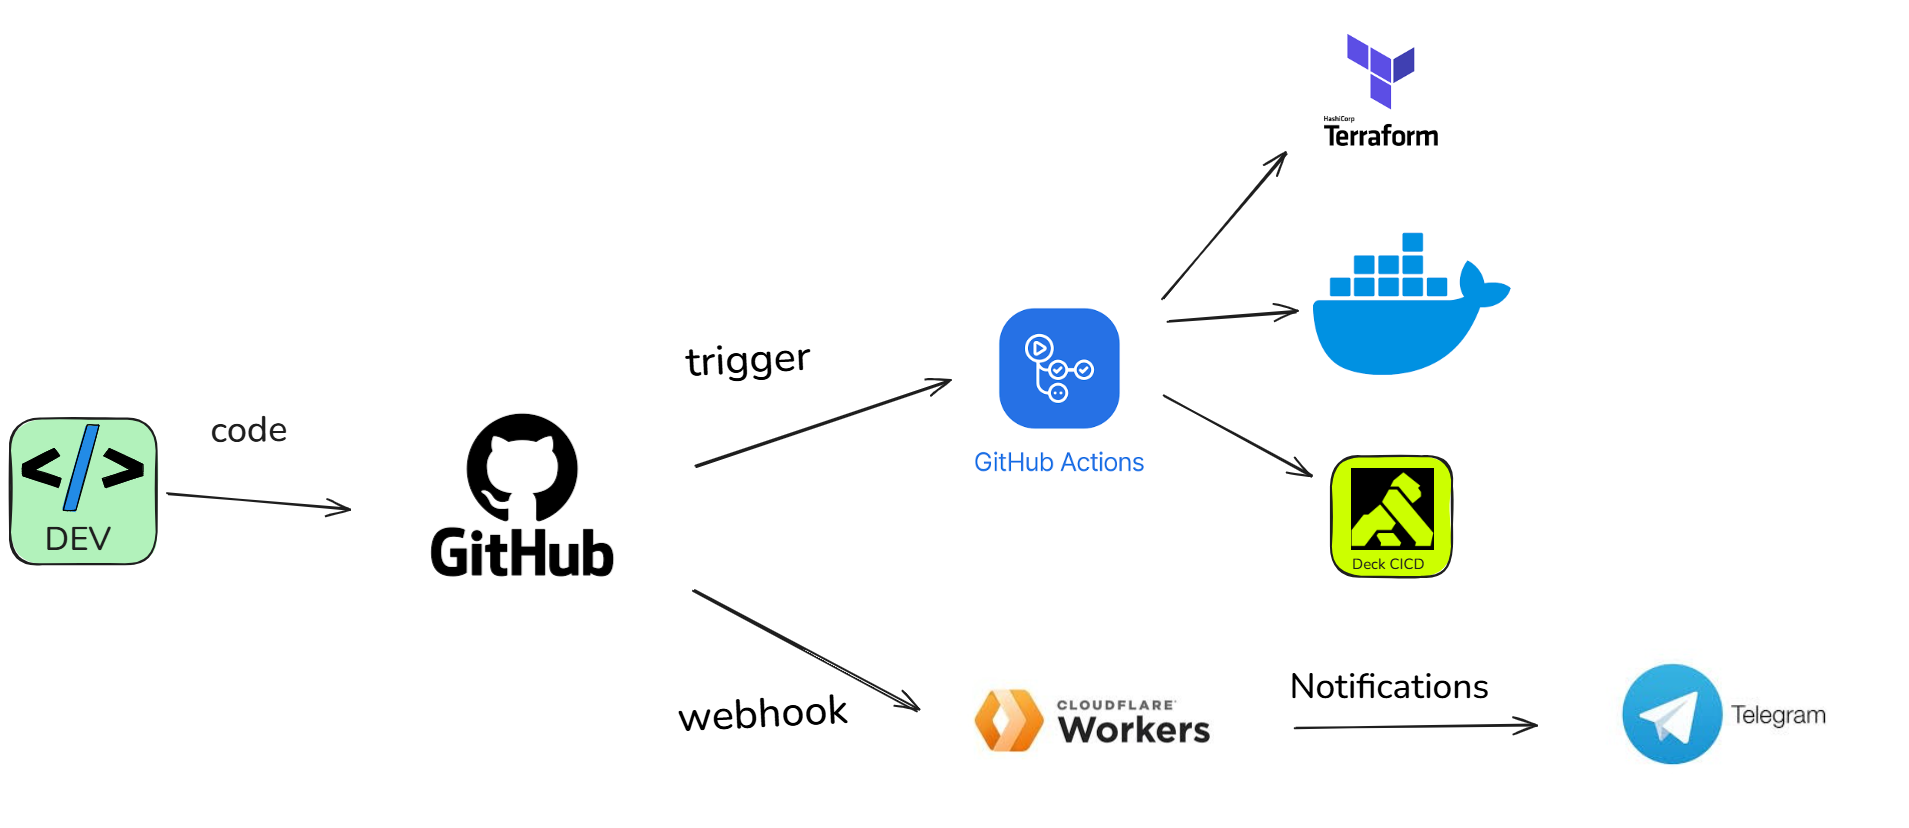
\includegraphics[scale = 0.2]{pictures/cicd-by-github-action.excalidraw.png}
\caption{Cấu hình chia nhỏ bí mật theo từng nhu cầu sử dụng trong doppler}
\end{figure}

\begin{block}{Ứng dụng trong đồ án}

Trong đồ án này,
hệ thống vừa sử dụng Github Action miễn phí của Github,
vừa sử dụng Self-hosted runner trên VPS.

\end{block}
